\chapter{Cmake}

\section{Overview}

Cmake is super old. It has more than 300 functions to use, but 250 should not be used in modern cmake projects. 
This makes it particularly difficult to learn. Many older tutorials are confusing, out-of-date.

Moreover, modern cmake makes it as readable as possible with modern functions. Thus, way easier to read than older
functions.

\section{Project Structure}

See basic project and intermediate project examples, in cmake udemy.


\begin{center}
    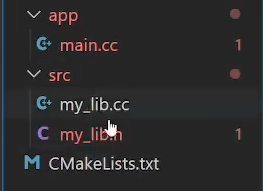
\includegraphics[width=2in]{cpp_tree1.png}
\end{center}


\begin{center}
    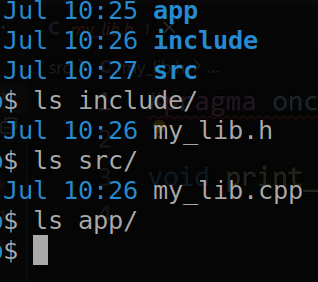
\includegraphics[width=2in]{cpp_tree2.png}
\end{center}

\subsection{App Directory}

Define everything important for the executable target, including its own CMakeLists.txt.

\subsection{Source Directory - src}

Define everything important for our library. When you have multiple libraries, create multiple directories in
src. As a naming convention, the subdirectory should have the same name as the library.

\begin{center}
    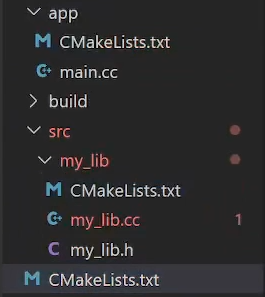
\includegraphics[width=2in]{cpp_tree3.png}
\end{center}

Don't forget to add a CMakeList in the src directory.


\begin{center}
    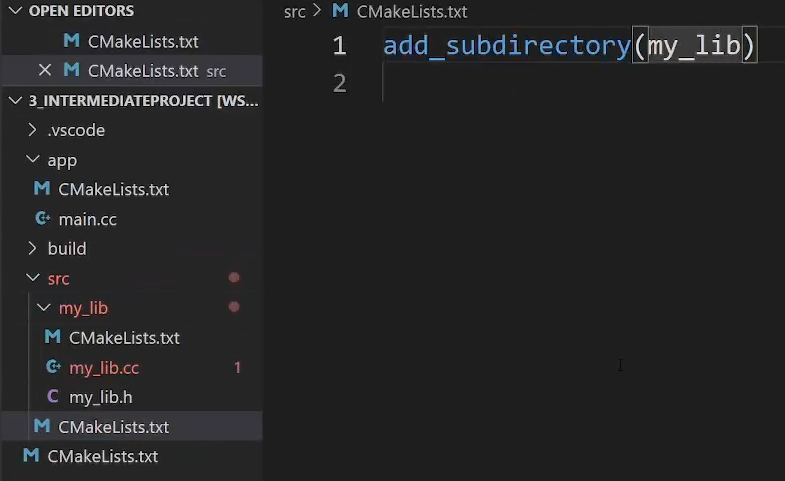
\includegraphics[width=4in]{cpp_tree4.png}
\end{center}

\subsection{CMake Default Paths}

Cmake has built-in paths to use. We use many in these notes.

\begin{verbatim}
# CMAKE_SOURCE_DIR is always the directory of the
# root CMakeLIsts.txt file
# our root directory

# CMAKE_BINARY_DIR is always our build directory
\end{verbatim}



\subsection{Template for Projects is Intermediate project}

Create a project builder based on the architecture of the intermediate project.


\section{Variables}

You can create variables for you executable or your libraries in the root CMakeLists.txt. The variables
will be usable in all add\_subdirectory chain at the end of the same document.

\begin{verbatim}
# set a variable for the library you want to use
# common synthax is capital letters.

# we reference Library in other CMakeLists files
# we change the Library name for LIBA

set(LIBA Library)

# where we used Library, write ${LIBA}


# we have used Hello for our executable name so far.
# we can change it as well.
set(HE Hello)

# where we used Hello, write ${HE}

add_subdirectory(src)
add_subdirectory(app)
\end{verbatim}


\subsection{Standard for cpp}

This is essential to have in your program. Otherwise, the compiler's default config will take the lead, with huge
variability between compiler versions!
In your root CMakeLists.txt file as well. This defines a variable and sets the standard to 17.

\begin{verbatim}
set(CMAKE_CXX_STANDARD 17)
set(CMAKE_C_STANDARD 98)
\end{verbatim}

\subsection{Standard Required}

Indicate that the compiler 100 pourcent implemented the language's standard.

\begin{verbatim}
set(CMAKE_CXX_STANDARD 17)
set(CMAKE_CXX_STANDARD_REQUIRED ON)
\end{verbatim}

\subsection{Compiler Extensions}

Some compilers have features that are not implemented in the Cpp standard. These features are extensions.
Some compilers allow you to use non-standard c code into a cpp program, even if they are not in the cpp standard.

\begin{verbatim}
set(CMAKE_CXX_STANDARD 17)
set(CMAKE_CXX_STANDARD_REQUIRED ON)
set(CMAKE_CXX_EXTENSIONS OFF)
\end{verbatim}

\subsection{If Statement}

Cmake has if statement. It even has string comparaison functions, to compare variable and create conditions.

\begin{verbatim}
option(COMPILE_EXECUTABLE "Whether to compile the executable" OFF)

add_subdirectory(src)

if (COMPILE_EXECUTABLE)
    add_subdirectory(app)
else()
    message("Without executable compiling")
endif()



\end{verbatim}


\subsection{Options}

You can set an option, the second argument is a simple comment for the reader (with no impact).

\begin{verbatim}
set(CMAKE_CXX_STANDARD 17)
set(CMAKE_CXX_STANDARD_REQUIRED ON)
set(CMAKE_CXX_EXTENSIONS OFF)

set(LIBA Library)
set(HE Hello)

option(COMPILE_EXECUTABLE "Whether to compile the executable" OFF)

add_subdirectory(src)

if (COMPILE_EXECUTABLE)
    add_subdirectory(app)
endif()


# to call the option from the command line

#$ cmake .. -DCOMPILE_EXECUTABLE=ON

# then you can switch it back OFF later

#$ cmake .. -DCOMPILE_EXECUTABLE=OFF
\end{verbatim}


\section{Makefile Shell Scripting}

Make is Cmake's ancestor. You can automate folder creation and files, just like any shell script would do. 

Make do not support space, use tabs.

\begin{verbatim}
prepare:
    rm -rf build
    mkdir build
    cd build

# to execute it

# $ make prepare
\end{verbatim}



\section{Project Software Toolkit}

\begin{verbatim}
Doxygen - create html documentation based on your codebase
Conan/VCPKG Packaging - How to install and use external libraries
Unit Testing
Code Coverage
CI Testing -- use all these tools in continuous integration, Github actions


We'll see how to create an html documentation based on your codebase
\end{verbatim}

\section{Installation Commands}

\begin{verbatim}
sudo apt-get update
sudo apt-get upgrade

# Mandatory
sudo apt-get install gcc g++ gdb
sudo apt-get install make cmake
sudo apt-get install git
sudo apt-get install doxygen
sudo apt-get install python3 python3-pip

# Optional
sudo apt-get install lcov gcovr
sudo apt-get install ccache
sudo apt-get install cppcheck
sudo apt-get install llvm clang-format clang-tidy
sudo apt-get install curl zip unzip tar

# for VSCODE

in extension, download franneck94 c/c++ extension pack
And the coding tools extension pack
Then, with command palette (in view), Config: generate C config file. It configures all tools the same as the
teacher's
\end{verbatim}

\section{Command Line Options}

\subsection{Generating a Project}

\begin{verbatim}
cmake [<options>] -S <path-to-source> -B <path-to-build>
\end{verbatim}

Assuming that a CMakeLists.txt is in the root directory, you can generate a project like the following.

\begin{verbatim}
mkdir build
cd build
cmake -S .. -B . # Option 1
cmake .. # Option 2

Assuming that you have already built the CMake project, you can update the generated project.

cd build
cmake .
\end{verbatim}

\subsection{Generator for GCC and Clang}

\begin{verbatim}
cd build
cmake -S .. -B . -G "Unix Makefiles" # Option 1
cmake .. -G "Unix Makefiles" # Option 2
\end{verbatim}

\subsection{Generator for MSVC}

\begin{verbatim}
cd build
cmake -S .. -B . -G "Visual Studio 16 2019" # Option 1
cmake .. -G "Visual Studio 16 2019" # Option 2
\end{verbatim}

\subsection{Specify the Build Type}

Per default, the standard type is in most cases the debug type.
If you want to generate the project, for example, in release mode you have to set the build type.

\begin{verbatim}
cd build
cmake -DCMAKE_BUILD_TYPE=Release ..
\end{verbatim}

\subsection{Passing Options}

If you have set some options in the CMakeLists, you can pass values in the command line.

\begin{verbatim}
cd build
cmake -DMY_OPTION=[ON|OFF] ..
\end{verbatim}

\subsection{Specify the Build Target (Option 1)}

The standard build command would build all created targets within the CMakeLists.
If you want to build a specific target, you can do so.

\begin{verbatim}
cd build
cmake --build . --target ExternalLibraries_Executable
\end{verbatim}

The target ExternalLibraries\_Executable is just an example of a possible target name.
Note: All dependent targets will be built beforehand.

\subsection{Specify the Build Target (Option 2)}


Besides setting the target within the cmake build command, you could also run the previously generated Makefile (from the generating step).
If you want to build the ExternalLibraries\_Executable, you could do the following.

\begin{verbatim}
cd build
make ExternalLibraries_Executable
\end{verbatim}


\section{Run the Executable}

After generating the project and building a specific target you might want to run the executable.
In the default case, the executable is stored in build/5\_ExternalLibraries/app/ExternalLibraries\_Executable, assuming that you are building the project 5\_ExternalLibraries and the main file of the executable is in the app dir.

\begin{verbatim}
cd build
./bin/ExternalLibraries_Executable
\end{verbatim}



\section{Configuration - Precompiling Information}

Create a configuration directory. With a config.hpp.in file.

\begin{center}
    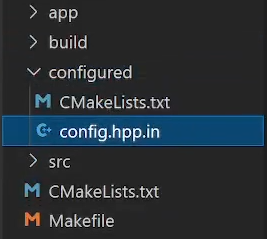
\includegraphics[width=2in]{conf.png}
\end{center}

In the CMakeLists.txt of this new configured directory.

\begin{verbatim}
configure_file(
    "config.hpp.in"
    # "${CMAKE_BINARY_DIR}" this is our build directory
                          # it is one of prebuilt directories in CMAKE
                          # thus, we reference it with CMAKE_BINARY_DIR
                          # we create an output for a config file, 
                          # in our build directory.

    # "${PROJECT_SOURCE_DIR}" # stores absolute path to project's root directory

    "${CMAKE_BINARY_DIR}/configured_files/include/config.hpp" ESCAPE_QUOTES 
\end{verbatim}

\subsection{Project Version Number}

In config.hpp.in

\begin{verbatim}
# @ cmake looks for and remplaces text between @@ this text @

#include <cstdint>
#include <string_view> 
static constexpr std::string_view project_name = "@PROJECT_NAME@";
static constexpr std::string_view project_version = "@PROJECT_VERSION@";
\end{verbatim}




\subsection{Sementic Versioning}

In version names: 1.0.0 . This is the first Major version (1). Incrementing the major version means
that the previous and the new codebase are not compatible at all. 2.0.0 have breaking changes with the 1.0.0 version.

The minor version 1.6.0, number 6 here, indicate that new features are available. Yet, nothing breaks between minor versions.

The patches are the last number, the last small fixes.

\begin{verbatim}
static constexpr std::int32_t project_version_major{@PROJECT_VERSION_MAJOR@};
static constexpr std::int32_t project_version_minor{@PROJECT_VERSION_MINOR@};
static constexpr std::int32_t project_version_patch{@PROJECT_VERSION_PATCH@};

#### Resulting file looks like.

#pragma once

#include <cstdint>
#include <string_view>

static constexpr std::string_view project_name = "CppProjectTemplate";
static constexpr std::string_view project_version = "1.0.0";

static constexpr std::int32_t project_version_major{1};
static constexpr std::int32_t project_version_minor{0};
static constexpr std::int32_t project_version_patch{0};
\end{verbatim}


\section{Sources and Headers}

When you have many libraries and many headers, create a variable for all of you headers. Then, reference this variable to include
everything. List all of your source files in my\_lib directory.

\begin{verbatim}
set(LIBRARY_SOURCES
     "my_lib.cpp"
     "my_lib2.cpp"
     ) # quotes are not mandatory, just preference.
set(LIBRARY_HEADERS
     "my_lib.h")

add_library(${LIBRARY_NAME} STATIC
    "./"
    "${CMAKE_BINARY_DIR}/configured_files/include")
\end{verbatim}

\subsection{Executables}

You can do the same thing if you generate many executables, I think. This would be in your app directory.

\begin{verbatim}
set(EXE_SOURCES
    "main.cpp")

add_exectable(${EXECUTABLE_NAME} ${EXE_SOURCES})
target_link)libraries(${ECEXUTABLE_NAME} PUBLIC ${LIBRARY_NAME})
\end{verbatim}


\section{Using External Libraries}


\subsection{Git Submodule - nlohman json}

Create an external directory. Our project looks like this:

\begin{center}
    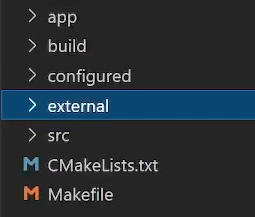
\includegraphics[width=2in]{external.png}
\end{center}

\begin{verbatim}
// make sure that your root folder is a git repo, git init

git submodule add https://github.com/nlogmann/json external/json

// it creates the json directory, when cloning the module in it.
\end{verbatim}

\subsection{Custom Cmake Functions}

In a cpp project, when you create your own cmake functions, they are stored in a Cmake directory. We just cloned a 
git repo in our external directory.

\begin{center}
    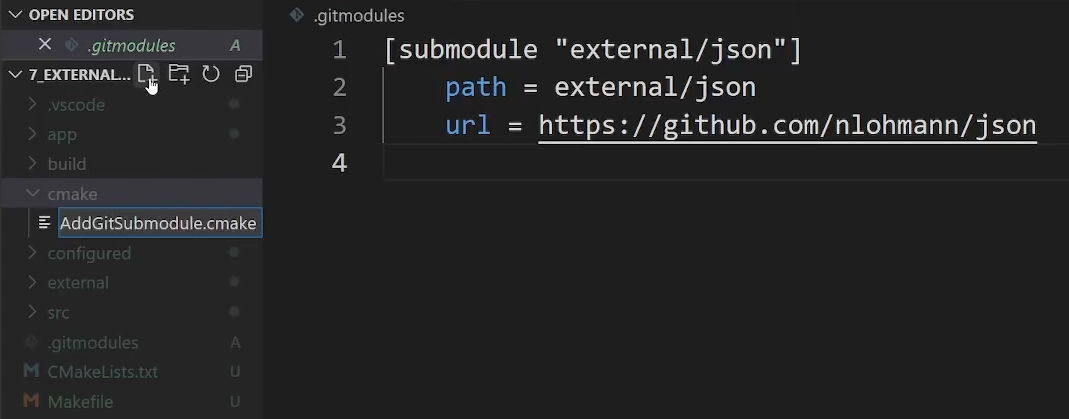
\includegraphics[width=4in]{add.png}
\end{center}

Now we create a AddGitSubmodule.cmake file. Inside, we define our function.

\begin{verbatim}
function(add_git_submodule dir) # our function takes one argument called dir
                                # this dir, is where the submodule is located
                                # making the add_ action possible.
        find_package(Git REQUIRED) # Git must be on your computer, or it
                                   # Error's out.
        if (NOT EXISTS ${dir}/CMakeLists.txt)
            execute_process (COMMAND ${GIT_EXECUTABLE}}
            submodule update --init --recursive -- ${dir}
                                                     # recursive is essential here
                                                     # If someone clones your project, 
                                                     # It automatically clones this submodules,
                                                     # It clones auto repos, inside your repo.
                                                            
            WORKING_DIRECTORY ${PROJECT_SOURCE_DIR}) # cmake saves some variable
                                                     # including the source dir
                                                     # of our project.
        endif()
        
        if (EXISTS ${dir}/CMakeLists.txt)
            message("Adding ${dir}/CMakeLists.txt")
            add_subdirectory(${dir})
        else
            message("Could not add ${dir}/CMakeLists.txt")
        endif()
endfunction(add_git_submodule)
\end{verbatim}


\subsection{Log example}

Here we are using an external library called log, with only two files, log.c and log.h . We have the library in our 
external directory. Plus, we have a CMakeLists.txt at the root of the external folder, taking care of the log library. 


\begin{center}
    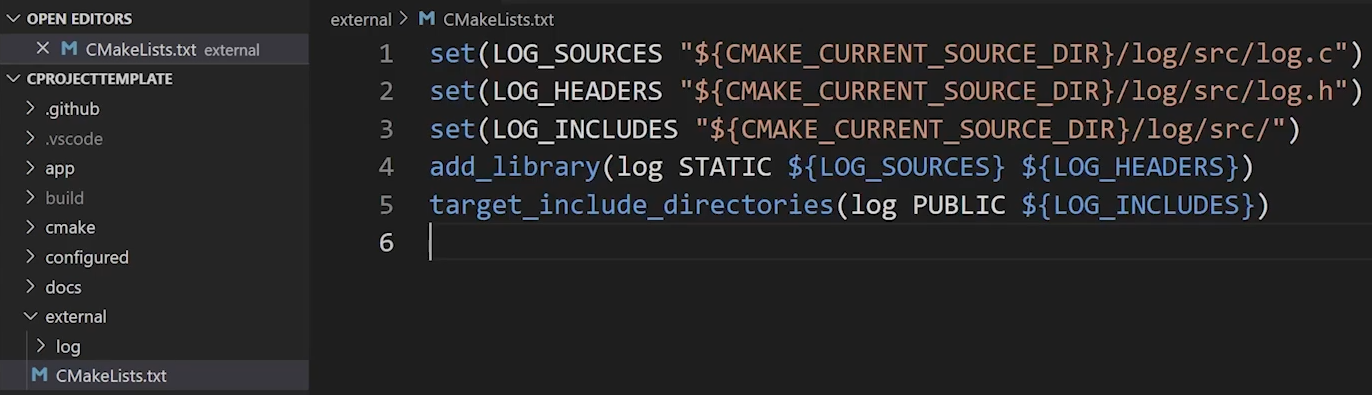
\includegraphics[width=5in]{loge.png}
\end{center}



\subsection{Call Your Own Functions}

In the source CMakeFiles.txt, knowing that we have a new git submodule. We add:


\begin{verbatim}
set(CMAKE_MODULE_PATH "${PROJECT_SOURCE_DIR}/cmake")
include(AddGitSubmodule) # includes indicates thats it a cmake module file.
                         # it will look where cmake modules are defined
                         # in our cmake dir


add_git_submodule(external/json) # this calls our custom function.

# In our app, we add this as well

set(EXE_SOURCES
    "main.cpp")

add_exectable(${EXECUTABLE_NAME} ${EXE_SOURCES})
target_link_libraries(${EXECUTABLE_NAME} PUBLIC
    ${LIBRARY_NAME}
    nlohmann_json) # this links the submodule with the executable

# In main.cpp, we add 

#include <nlohman/json.hpp>
\end{verbatim}


\subsection{Fetch Content - External Libraries}

We have the gitmodule example, but modern CMake has a great fetching feature. Our root CMakelLists.txt will look like this, 

\begin{verbatim}
...

set(CMAKE_MODULE_PATH "${PROJECT_SOURCE_DIR}/cmake/")
include(AddGitSubmodule)


include(FetchContent)  # built-in library or file
                       # including it gives access to features

FetchContent_Declare() # Declare which github repository we would like to use
FetchContent_MakeAvailable() # will load this library in our cmake project.


                       # I want to use github.com/nlohmann/json
                       # any Gitlab is also possible
                       # I can do:
FetchContent_Declare(
    nlohmann_json      # since this repo is a cmake project,
                       # look at the project's root CMakeLists.txt file
                       # you will the name of the project, to enter here 
                       # see next image

    GIT_REPOSITORY https://github.com/nlohmann/json
    GIT_TAG v3.11.2    # the version I want to use
    GIT_SHALLOW TRUE)  # The function won't clone the repo recursively

                       # With this function, the git repository will be cloned in  
                       # our cloned repository.
                       # And it needs to be a cmake project.

                       # if it is not a cmake project, use the AddGitSubmodule method shown.
FetchContent_MakeAvailable(nlohmann_json) # will load this library in our cmake project.
\end{verbatim}

\begin{center}
    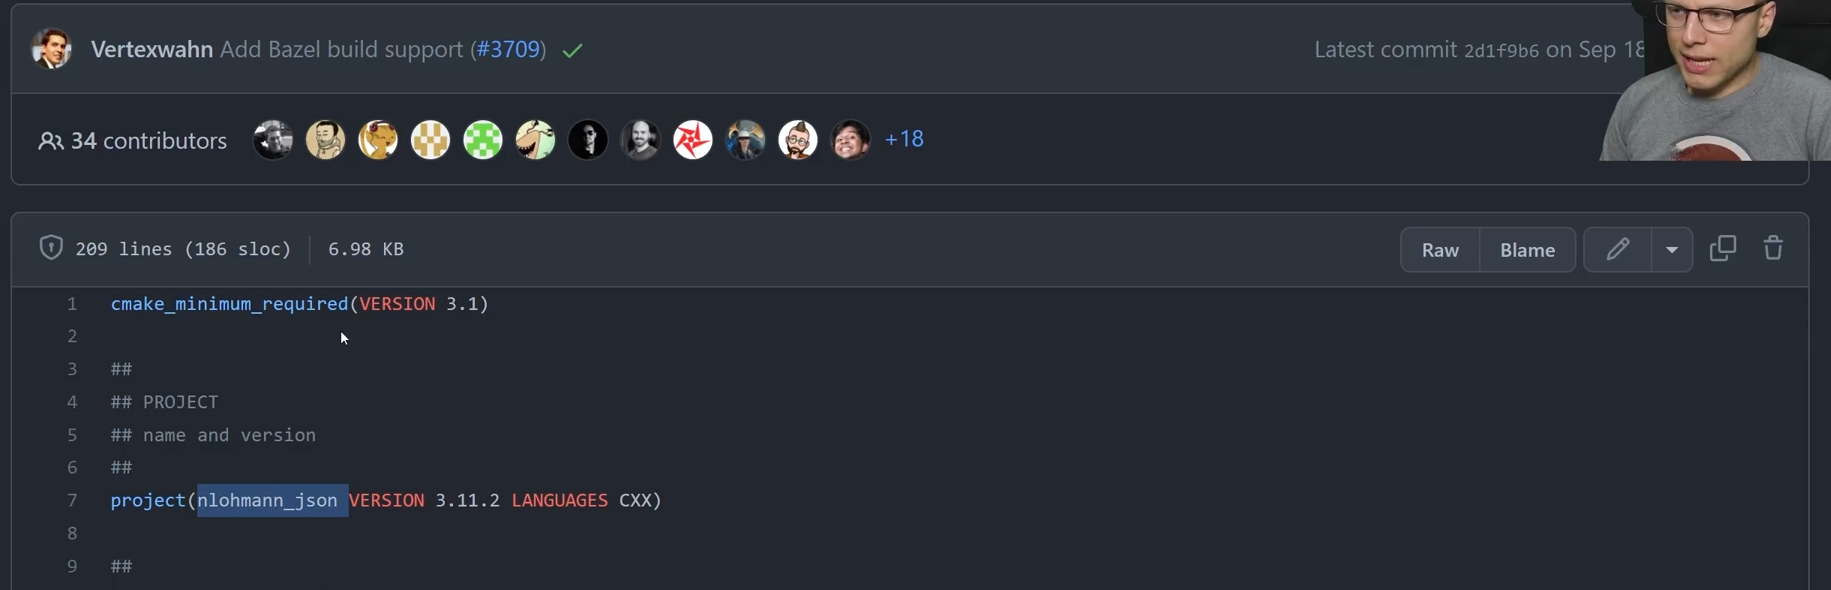
\includegraphics[width=5in]{json_n.png}
\end{center}


\subsection{FMT}

The best library to easily format strings in cpp.

\begin{verbatim}
FetchContent_Declare(
    fmt
    GIT_REPOSITORY https://github.com/fmtib/fmt
    GIT_TAG 9.1.0
    GIT_SHALLOW TRUE)
FetchContent_MakeAvailable(fmt)
\end{verbatim}

\subsection{spdlog}

The best fast logging library for cpp.

\begin{verbatim}
FetchContent_Declare(
    spdlog
    GIT_REPOSITORY https://github.com/gabime/spdlog
    GIT_TAG v1.11.0
    GIT_SHALLOW TRUE)
FetchContent_MakeAvailable(spdlog)
\end{verbatim}

\subsection{Cxxopts}

The best library to work with command line arguments in cpp. From the received arguments, to any other type.
The equivalent of the argument parser in python.

\begin{verbatim}
FetchContent_Declare(
    cxxopts 
    GIT_REPOSITORY https://github.com/jaroo2783/cxxopts
    GIT_TAG v3.0.0
    GIT_SHALLOW TRUE)
FetchContent_MakeAvailable(cxxopts)
\end{verbatim}

\subsection{Catch2}

The best Unit Testing library, seen further below.

\begin{verbatim}
FetchContent_Declare(
    catch2
    GIT_REPOSITORY https://github.com/catchorg/Catch2
    GIT_TAG v2.13.9  # teacher recommended this version, not the latest.
    GIT_SHALLOW TRUE)
FetchContent_MakeAvailable(catch2)
\end{verbatim}


\subsection{Include All Libraries in root CMakeListstxt}

Refer to Final project Template seen in the course. Modifying the CMakeLists.txt in our my-lib directory.

\begin{center}
    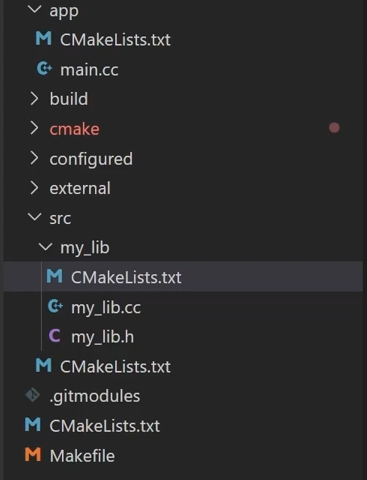
\includegraphics[width=2in]{final_p.png}
\end{center}

\begin{verbatim}
set(LIBRARY_SOURCES
    "my_lib.cpp")
set(LIBRARY_HEADERS
    "my_lib.h")
set(LIBRARY_INCLUDES
    "./"
    "${CMAKE_BINARY_DIR}/configured_files/include")

add_library(${LIBA} STATIC
    ${LIBRARY_SOURCES}
    ${LIBRARY_HEADERS})
target_include_directories(${LIBA} PUBLIC
    ${LIBRARY_INCLUDES})
target_link_libraries(${LIBA} PUBLIC
                                        # Naming convention is project_name::library_name
                                        # see next image, to find library_name in CMake project
                                        # on github
    
    nlohmann_json::nlohmann_json
    fmt::fmt
    spdlog::spdlog
    catch2::catch2
    cxxopts::cxxopts                    # not always the same

    )
\end{verbatim}

When this is set-up, and we reconfigure our cmake project, the repository will be cloned in a \_deps directory. This includes
a build, subbuild and src directory for all dependencies. Don't worry about it for now.

\begin{center}
    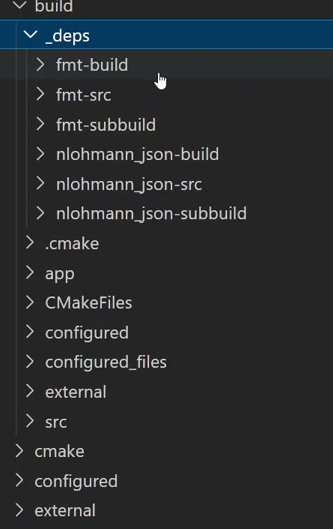
\includegraphics[width=2in]{deps.png}
\end{center}


\subsection{Include all Libraries in App Main.cpp}

It is tricky to include the libraries files in main. Some have directories, some do not.

\begin{verbatim}
#include <iostream>

#include <cxxopts.hpp>
#include <nlohman/json.hpp>
#include <fmt/format.h>
#include <spdlog/spdlog.h>
#include <catch2>

#include "my_lib.h"
#include "config.hpp"

int main() {
    ...
    std::cout << "CXXOPTS: # chose any included lib, to prove you have access to their info

    << CXXOPTS__VERSION_MAJOR << "."
    << CXXOPTS__VERSION_MINOR << "."
    << CXXOPTS__VERSION_PATCH << "." # if you have access to these variable, 
                                     # you have successfully imported and configure the lib
                                     # for you project.

    ...

}
\end{verbatim}


\subsection{Git Submodules vs Fetch Content}

If the repo is not a CMakeProject, you should use Git Submodules. Valid for GitHub and GitLab. In this case, 
define its own library target, I think. Not explained in detail.

If it is a CMake project on GitHub or Gitlab, use FetchContent. It is easier to use, you don't need to mess with header
libraries or anything. We can simply use the makeAvailable and prepare function.

The instructor highly recommends FetchContent!


\chapter{CMake Package Managers}

\section{CPM - Cmake Package Manager}

There are a few ways to include external libraries in you project. Git submodules, fetch content and packages managers such as
Cmake Package Manager.

On CPM's github page, click Releases. Pick the latest release, download the CPM.cmake file and copy it to your project's
cmake directory.

\begin{center}
    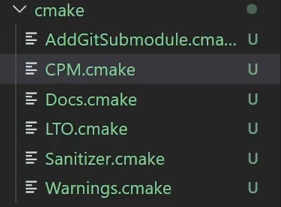
\includegraphics[width=2in]{cpm1.png}
\end{center}


\subsection{CPM configuration in root CMakeLists.txt}

Add an option in your root CMakeLists.txt.
Since the course's project has two different ways to import external libraries,
we will have an option for cpm and for fetch content.
We shouldn't use multiple tools at the same time. Thus, code
an if statement to use one or the other fetching method.

\textbf{Every external libraries used under CPM need to be github CMake projects, which 95 pourcent are.
It shouldn't be a problem}.


\textbf{Under the hood, CPM uses fetchcontent}. Therefore, the linking,
in the src/my\_lib/CMakeLists.txt file target\_link\_libraries function, 
can keep the fetchcontent synthax of nlohman\_json::nlohman\_json.


\begin{verbatim}
option(USE_CPM "Whether to use CPM" ON)

if(USE_CPM)
    message(STATUS "Using Cmake Package Manager")
    include(CPM)            # this includes the cpm.cmake file
    


                # "gh" cpm will look at github
                # "gh:nholmann" username
                # "gh:nholmann/json" repository name
                # "gh:nholmann/json#v3.11.2" version number 

    cpmaddpackage("gh:nholman/json#v3.11.2")    # This is CPM's defined function
    cpmaddpackage("gh:fmtlib/fmt#9.1.0")
    cpmaddpackage("gh:gabime/spdlog#v1.11.0")
    cpmaddpackage("gh:jarro2783/cxxopts#v3.1.1")
    cpmaddpackage("gh:cathorg/Catch2#v2.13.9")

else()
    message(STATUS "Using FetchContent")

    FetchContent_Declare(
        nlohmann_json      
        GIT_REPOSITORY https://github.com/nlohmann/json
        GIT_TAG v3.11.2    
        GIT_SHALLOW TRUE)  
    FetchContent_MakeAvailable(nlohmann_json) # will load this library in our cmake project.

    FetchContent_Declare(
        fmt
        GIT_REPOSITORY ...

endif()
\end{verbatim}

\section{Conan}

A package manager for cmake projects, alternatives to CPM and fetchcontent. CPM and fetchcontent localy
clones github repositories in your build directory. Then they compile the library locally, on your machine. 


Conan has a different approach. In an online database, pre-compiled repositories are available.
Conan downloads these. It depends on the compiler, but it generally saves compilation time.
No need to compile locally.

Conan binaries are compiled as release builds, not as debug builds.

A drawback for Conan is the binary updates. There are many configuration possible, and many updates
to keep track of. Therefore, many popular libraries won't have a compiled version for our machine's
configuration. Too many possibilities, Conan can't keep up with updates.

\subsection{Conan Installation}

\begin{verbatim}
Official installation guide is [here](https://docs.conan.io/2/).

The conan database is [here](https://conan.io/center/).

1. Install Python (3.7+)
2. Type ``pip install --user -U conan`` into the terminal
   1. Unix: Append conan to the PATH by: ``source ~/.profile``
3. Run: $ conan

4. $ conan profile detect --force
5. $ conan profile path default
\end{verbatim}


\subsection{Conan Configuration in root CMakeLists.txt}

There is a pattern here, when you want to use something new in your cmake project,
set an option in the CMakeLists.txt file first.

Since the course shared examples for GitSubmodules, FetchContent, CPM and Conan,
we have a large if statement in our root CMakeLists.txt. In a regular project, 
select the tool you want, you wouldn't need the if.

\begin{verbatim}
option(USE_CONAN "Whether to use CPM" ON)

if(USE_CPM)
    ...
elseif(USE_CONAN)
    message(STATUS "Using Conan")
    include(${CMAKE_BINARY_DIR}/conan_toolchain.cmake  
                                # This is generated by a conan command
                                # in the conanfile.py (generate)
                                # including it in advance here.
    find_package(nlohmann_json REQUIRED)
    find_package(fmtlib REQUIRED)
    find_package(spdlog REQUIRED)
    find_package(cxxopts REQUIRED)
    find_package(Catch2 REQUIRED)

else()
    FetchContent_Declare(
        ...
\end{verbatim}

\subsection{Conanfile.py}

To configure conan, create a conanfile.py in your root directory.

\begin{center}
    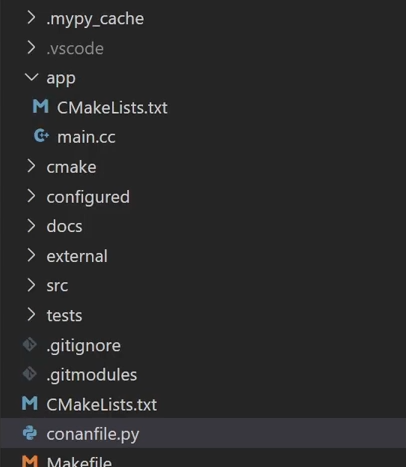
\includegraphics[width=2in]{conanfile.png}
\end{center}

\begin{verbatim}
from conan import ConanFile
from conan.tools.cmake import CMakeToolchain

class CompressorRecipe(ConanFile):
    settings = "os", "compiler", "build_type", "arch"
    generators = "CMakeDeps"

    def requirements(self):
        self.requires("nlohman_json/3.11.2")    # look at conan's database
                                                # to see which pre-compiled
                                                # versions are available
        self.requires("fmt/9.1.0")
        self.requires("spdlog/1.11.0")
        self.requires("catch2/2.13.9")
        self.requires("cxxopts/3.1.1")

    def generate(self):                         # this function generates the
                                                # conan_toolchain.cmake file
        tc = CMakeToolchain(self)
        tc.user_presets_path = False
        tc.generate()
\end{verbatim}

\subsection{Conan Debug Build}

Conan has release binaries by default, you have to tweak settings for you debug build.
To automatize conan's debug management, the instructor changed its makefile script.


\begin{verbatim}
conan_d:    # for conan debug
    rm -rf build
    mkdir build
    cd build && conan install .. -s build_type=Debug =s compiler.cppstd=17 --output-folder=. --build missing
                                -s               # for settings change
                                -- build missing 
                                                 # build binaries where no compiled version are available

conan_r:    # for conan release
    rm -rf build
    mkdir build
    cd build && conan install .. -s build_type=Release -s compiler.cppstd=17 --output-folder=. --build missing



### With this, run

$make conan_d
$make conan_r
\end{verbatim}  


\subsection{Conan Generated File}

Conan generates many files in your build directory, based on our configurations. Yet, no need to worry about them, conan
will deal with them.


\begin{center}
    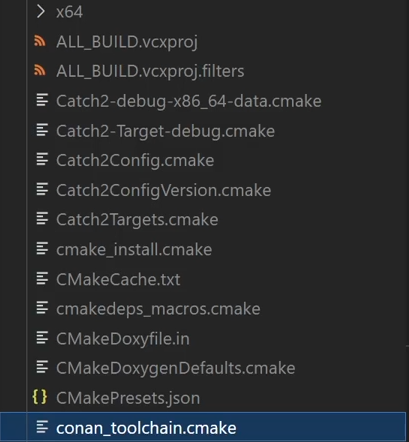
\includegraphics[width=2in]{conan2.png}
\end{center}




\subsection{VCPKG}

\section{Dependency Graphs}

In a makefile, or any script, use the command --graphviz. Dependency and prepare are the flag needed to run the command.

\begin{verbatim}
dependency:
    cd build && cmake .. --graphviz=grap.dot && dot -Tpng graph.dot -o grapImage.png
                        // not yet an image when .dot
                        // but easy to transform
prepare:
    rm -rf build
    mkdir build
                        // unrelated to dependency graph.
\end{verbatim}

The house symbol is the executable. Rectangle are external libraries. Losanges shapes are internal libraries.

\begin{center}
    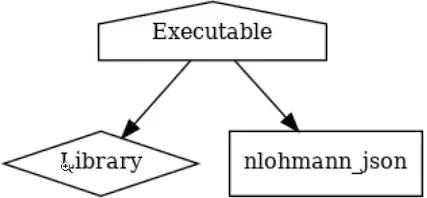
\includegraphics[width=2in]{graph.png}
\end{center}

Towards the end of the course, the graph was more complex.

\begin{center}
    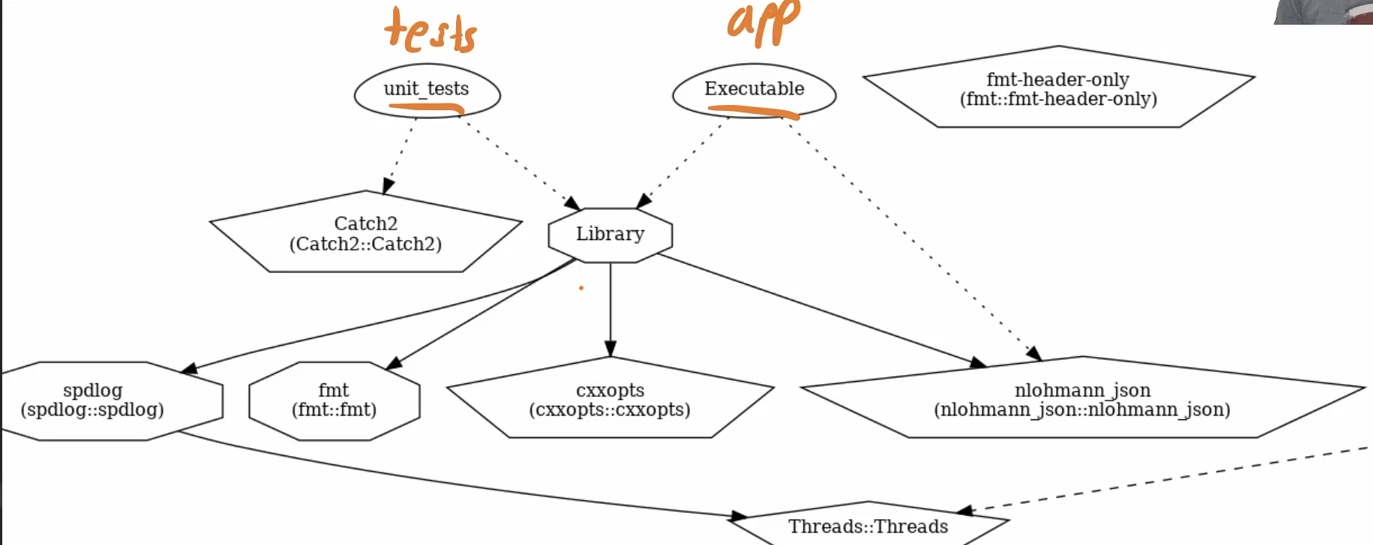
\includegraphics[width=5in]{graph3.png}
\end{center}



\section{Doxygen Documentation}

Generate html documentation for our code. For example, for our library. The course has a vscode extention: Doxygen Documentation Generator.

\subsection{Vscode Extension}

The extention generates documentation base on this synthax.

\begin{verbatim}
#include <iostream>

#include <nlohmann/json.hpp>
#include "my_lib.h"

/**
 * @brief Prints out hello world and tests the JSON lib.
 *
 *
 */
\end{verbatim}

\subsection{Doxygen Command Line}

Doxygen is looking for a doxy file, a config file. Generate a doxy file with doxygen -g.
In it, fill information on the project, name, version,  path to source files, etc. It will generate better html file with the information.
In the docs directory.

\begin{center}
    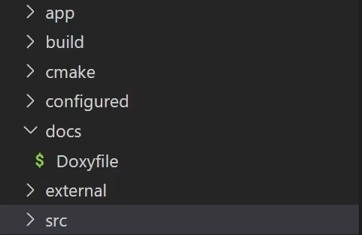
\includegraphics[width=2in]{dox.png}
\end{center}

\begin{verbatim}
# Configuration for Doxygen for use with CMake
# Only options that deviate from the default are included
# To create a new Doxyfile containing all available options, call `doxygen -g`

#---------------------------------------------------------------------------
# Project related configuration options
#---------------------------------------------------------------------------
DOXYFILE_ENCODING       = UTF-8
PROJECT_NAME            = "C++ Project Template"
PROJECT_NUMBER          = 1.0
PROJECT_BRIEF           =
PROJECT_LOGO            =
OUTPUT_DIRECTORY        = ./
OUTPUT_LANGUAGE         = English
MARKDOWN_SUPPORT        = YES

#---------------------------------------------------------------------------
# Build related configuration options
#---------------------------------------------------------------------------
EXTRACT_ALL             = YES
RECURSIVE               = YES
GENERATE_HTML           = YES
GENERATE_LATEX          = NO

#---------------------------------------------------------------------------
# Configuration options related to the input files
#---------------------------------------------------------------------------
INPUT                  =    ../src \
INPUT                       ../include
INPUT_ENCODING         = UTF-8
FILE_PATTERNS          = *.c \
                         *.cc \
                         *.cpp \
                         *.c++ \
                         *.h \
                         *.hpp \
                         *.h++ \
                         *.md \
                         *.dox \
                         *.doc \
                         *.txt
\end{verbatim}

When ready, generate the html with the command Doxygen, inside the docs folder (where the doxyfile is located). It creates an html dir.
it has the index.html automatically. The webpage looks like this:


\begin{center}
    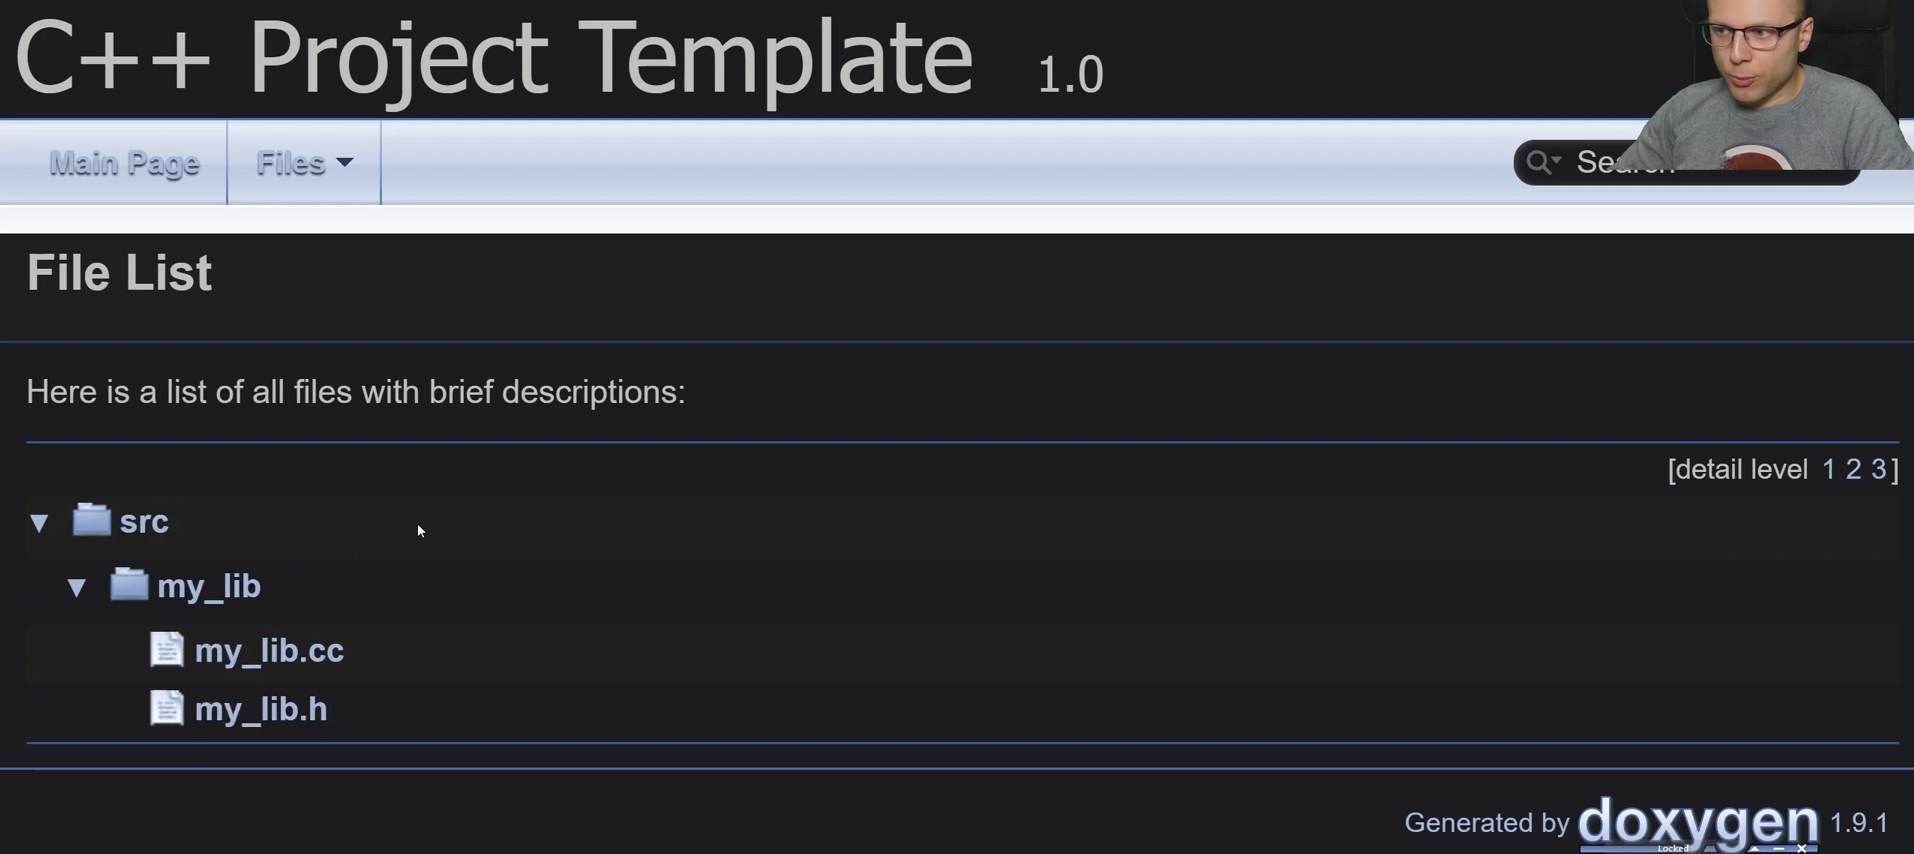
\includegraphics[width=5in]{dox2.png}
\end{center}


\subsection{Document Custom Target}

We need to add the documentation to our cmake project.

\begin{center}
    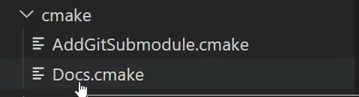
\includegraphics[width=3in]{doccmake.png}
\end{center}

In our root CMakeLists.txt, we add.

\begin{verbatim}
include(AddGitSubmodule)
include(FetchContent)
include(Docs)               # this is our new dir.

\end{verbatim}


\subsection{Doc.cmake}

Cmake needs to find Doxygen, because we are using it for our docs. In Docs.cmake,

\begin{verbatim}
find_package(Doxygen)
if (DOXYGEN_FOUND)
    add_custom_target( # This is just an utility target
                       # With it, we can interact with it, 
                       # in the terminal
    docs
    ${DOXYGEN_EXECUTABLE}
    WORKING_DIRECTORY ${CMAKE_SOURCE_DIR}/docs

                       # CMAKE_SOURCE_DIR is always the directory of the
                       # root CMakeLIsts.txt file
                       # our root directory

                       # CMAKE_BINARY_DIR is always our build directory
endif()
\end{verbatim}

Now Documentation can be built seperately, independently of the main project app built process.

\section{Catch2 - Unit Testing}

\subsection{Function testing example}

Adding Unit test to our codebase, with the catch2 library. Unit tests are useful to test functions from the library.

There is a tutorial on the github catch2 page. As an example, it provides this factorial function example, to try.


\begin{verbatim}
unsigned int factorial( unsigned int number ) {
    return number <= 1 ? number : factorial(number-1)*number;
}

// the instructor changes it to

std::uint32_t factorial(std::unint32_t number)
{

    return number <= 1 ? number : factorial(number-1) * number;

}
\end{verbatim}


\subsection{Test Directory}

To introduce unit testing, we create a new directory: tests.

\begin{center}
    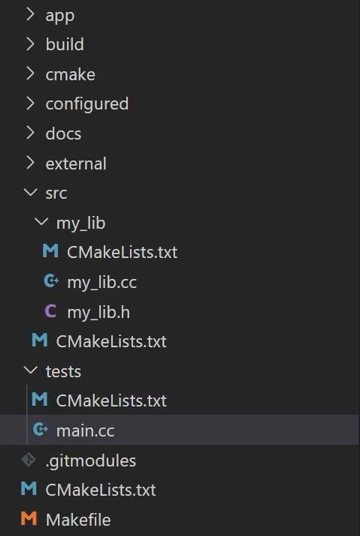
\includegraphics[width=2in]{tests.png}
\end{center}

In our root CMakeLists.txt.  

\begin{verbatim}
add_subdirectory(configured)
add_subdirectory(external)
add_subdirectory(src)
add_subdirectory(app)
add_subdirectory(tests) # adding tests
\end{verbatim}

\textbf{The idea is to have our main executable, our library(lib) and our unit test executable. The main and the Unit
executable we'll both use our library, but we will test with Unit. Unit will test if all our implemented functions work without bugs.}


\subsection{Tests Set-up, CMakeLists.txt}

\begin{verbatim}
set(TEST_MAIN "unit_tests")        # this is the name of our testing executable
set(TEST_SOURCES "main.cpp")       # Here, the tests are in one file only
                                   # It could be divided into more files
                                   # Header files for example
set(TEST_INCLUDES "./")
add_executable(${TEST_MAIN} ${TEST_SOURCES})
target_include_directories(${TEST_MAIN} PUBLIC ${TEST_INCLUDES})
target_link_libraries(${TEST_MAIN} PUBLIC ${LIBA} Catch2::Catch2)

                                   # Our library is linked, LIBA
                                   # This is how we will test it
\end{verbatim}


\subsection{Defining Tests}

To test the factorial function, this is the test definition given as example.

\begin{verbatim}
#define CATCH_CONFIG_MAIN // This tells Catch to provide a main() - only do this in one file
                          // No need to write int main() {}, this does it. 
#include "catch2/catch.hpp"

#include "my_lib.h"       // Will be called in my_lib.h

TEST_CASE( "Factorials are computed", "[factorial]" ) {
    REQUIRE( Factorial(1) == 1);
    REQUIRE( Factorial(2) == 2);
    REQUIRE( Factorial(3 == 6);
    REQUIRE( Factorial(10 == 362880 );
}

This function needs to be called in my_lib.h

std::uint32_t factorial(std::uint32_t number);
\end{verbatim}


\subsection{Command Line Testing Option}

It is convenient to have a command line option to activate or deactivate our testing build. In our root CMakeLists.txt
file, we add an option. In our CMakeLists.txt in the tests directory, we add an if statement. 

\begin{verbatim}
option(ENABLE_TESTING "Enable a Unit Testing Build" ON) 

# in tests directory's CMakeLists.txt

if (ENABLE_TESTING)
    set(TEST_MAIN "unit_tests")
    set(TEST_SOURCES "main.cpp")
    set(TEST_INCLUDES "./")

    add_executable(#{TEST_MAIN} ${TEST_SOURCES})
    target_include_directories(${TEST_MAIN} PUBLIC ${TEST_INCLUDES})
    target_link_libraries(${TEST_MAIN} PUBLIC ${LIBA} Catch2::Catch2)
endfi()
\end{verbatim}


\subsection{On Testing Libraries in General}

The specific words (Test\_case, require, etc.) may vary a bit, but they all have the same logic. When you are familiar with one, 
you will be able to use another testing library.

\begin{verbatim}
You have a test case, 

TEST_CASE()

You can give it a name and a short-name(abbriviated)

TEST_CASE( "Factorials are computed", "[factorial]" )

you can test a function with a keyword like require, or require_equal. Giving an input, the result should be. 
REQUIRE( factorial(0) == 0)
\end{verbatim}

\section{Public, Interface and Private}

Public and private is similar to OOP public and private keywords in classes.

\subsection{Different Linking Types}

\begin{verbatim}
add_library(A ...)
add_library(B ...)
add_library(C ...)
\end{verbatim}

\subsection{Public}

Here, fmt can be used in the library of A. 

\begin{verbatim}
target_link_libraries(A PUBLIC fmt)

target_link_libraries(C PUBLIC/PRIVATE A)
target_link_libraries(C PUBLIC/PRIVATE A)
\end{verbatim}

When A links fmt as PUBLIC, it says that A uses fmt in its implementation, and fmt is also used in A's public API.
Hence, C can use fmt since it is part of the public API of A.

\subsection{Private}

Using PRIVATE does not make the library available in the target's public API. Instead, it is part of a private API.
When B links in spdlog as PRIVATE, it is saying that B uses spdlog in its implementation,
but spdlog is not used in any part of B's public API. 

\begin{verbatim}
target_link_libraries(B PRIVATE spdlog)

target_link_libraries(C PUBLIC/PRIVATE B)
\end{verbatim}

Any code that makes calls into B would not need to refer directly to anything from
spdlog.


In a professional setting, you want to keep certain aspect of you project private. Hence, this option to consider.

\subsection{Interface}

In general, used for header-only libraries. That is, libraries where you don't need to compile anything. They do not have
any compilation logic in them.

\begin{verbatim}
add_library(D INTERFACE)
target_include_directories(D INTERFACE {CMAKE_CURRENT_SOURCE_DIR}/include)

# this only links something to the executable, I think. No compilation logic.
\end{verbatim}



\section{Different Library Types}

\subsection{Library}

A binary file that contains information about code.
A library cannot be executed on its own.
An application utilizes a library.

A library must be build too, if it is used by an executable.

\begin{verbatim}
cmake --build . --target Library
cmake --build . --target Executable // it is dependent to the Library build!
\end{verbatim}

\subsection{Shared}

\begin{verbatim}
Linux: *.so
MacOS: *.dylib
Windows: *.dll
\end{verbatim}

Shared libraries reduce the amount of code that is duplicated in each program that makes use of the library, keeping the binaries small.
Shared libraries will however have a small additional cost for the execution.
In general the shared library is in the same directory as the executable.

\subsection{Static}

\begin{verbatim}
Linux/MacOS: *.a
Windows: *.lib
\end{verbatim}

Static libraries increase the overall size of the binary, but it means that you don't need to carry along a copy of the library that is being used.
As the code is connected at compile time there are not any additional run-time loading costs.

\section{Adding Compiler Warnings}

You can pull certain warnings for a particular target. We can activate them based on the operating system and on the compiler.
We can trigger certain set of compiler checks. In this course, we had two targets: the library target and the executable target.

In the cmake directory, add Warnings.cmake. 


\begin{center}
    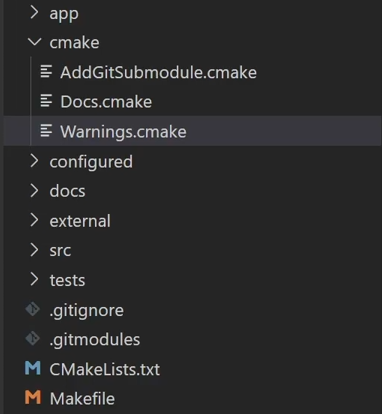
\includegraphics[width=2in]{warnings1.png}
\end{center}

\begin{verbatim}
function(target_set_warnings TARGET ENABLE ENABLED_AS_ERRORS)
    if (NOT ${ENABLED})
        message(STATUS "Warnings disabled for: ${TARGET}")

    set(MSCV_COMPILER
        /WA4
        /permissive-)

    set(CLANG_COMPILER
        -Wall
        -Wextra
        -Wpedantic)

    set(GCC_WARNINGS ${CLANG_WARNINGS})

    if(${ENABLED_AS_ERRORS}}
        set(MSCV_WARNINGS ${MSVC_WARNINGS} /WX) # We need to append to our MSVC compiler
                                                # We append /WX

        set(CLANG_WARNINGS ${CLANG_WARNINGS} -Werror)
                                                # We append -Werror
        set(GCC_WARNINGS ${GCC_WARNINGS} -Werror)
    endif()

    if(CMAKE_CXX_COMPILER_ID MATCHES "MSVC")
        set(WARNINGS ${MSVC_WARNINGS})
    elseif(CMAKE_CXX_COMPILER_ID MATCHES "CLANG")
        set(WARNINGS ${CLANG_WARNINGS})
    elseif(CMAKE_CXX_COMPILER_ID MATCHES "GNU")
        set(WARNINGS ${GCC_WARNINGS})
    endif()

    target_compile_options(${TARGET} PRIVATE ${WARNINGS})
    message(STATUS ${WARNINGS})

endfunction(target_set_warnings TARGET)
\end{verbatim}

\subsection{Check user's Compiler}

\begin{verbatim}
if(CMAKE_CXX_COMPILER_ID MATCHES "MSVC")
    set(WARNINGS ${MSVC_WARNINGS})
elseif(CMAKE_CXX_COMPILER_ID MATCHES "CLANG")
    set(WARNINGS ${CLANG_WARNINGS})
elseif(CMAKE_CXX_COMPILER_ID MATCHES "GNU")
    set(WARNINGS ${GCC_WARNINGS})
endif()
\end{verbatim}


\subsection{Warnings Root CMakeLists Options}

We just created a function to check the user's compiler and set compilation warnings.
Now create options in the root CMakeFilelists.txt.

\begin{verbatim}
option(ENABLE_WARNINGS "Enable warnings" ON)
option(ENABLE_WARNINGS_AS_ERRORS "Enable warnings as errors" ON)

    ...

if(ENABLE_WARNINGS)
    include(Warnings) # include the newly created Warnings.cmake file
endif()
\end{verbatim}


\subsection{Executable Target Enable Warnings}

There are two targets that can have compilation warnings, our library and our executable (our app). We have to 
add warning conditionals in both of their CMakeLists.txt file.

\begin{verbatim}
if(${ENABLE_WARNINGS})
    target_set_warnings(
        ${HE}       # this is our executable / app name,
                    # passed as argument in our created warnings function
        ${ENABLE_WARNINGS}
        ${ENABLE_WARNINGS_AS_ERRORS})
endif()

# for the lib CMakeLists.txt

if(${ENABLE_WARNINGS})
    target_set_warnings(
        ${LIBA}       # this is our library target name,
                      # passed as argument in our created warnings function
        ${ENABLE_WARNINGS}
        ${ENABLE_WARNINGS_AS_ERRORS})
endif()
\end{verbatim}

You don't have to have warnings as error for all targets, but you should have compilation warnings for all of them.

\section{Sanitizers}

Use sanitizers to find memory links or memory problems in your code. Sanitizers are used at runtime. 
Thus, it happens after compilation. Clang-tidy is a static linter, it finds problems before compilation!  

In order, you have clang-tidy before compilation, 
compiler warnings during compilation and sanitizers at runtime (after compilation).

In our root CMakeLists.txt, we add

\begin{verbatim}
option(ENABLE_SANITIZE_ADDR "Enable warnings" ON)
option(ENABLE_SANITIZE_UNDEF "Enable warnings" ON)


if(ENABLE_SANITIZE_UNDUF OR ENABLE_SANITIZE_ADDR)
    include(Sanitizers) # include a Sanitizers.cmake file
                        # same as Warnings.cmake file
endif()

\end{verbatim}

\begin{center}
    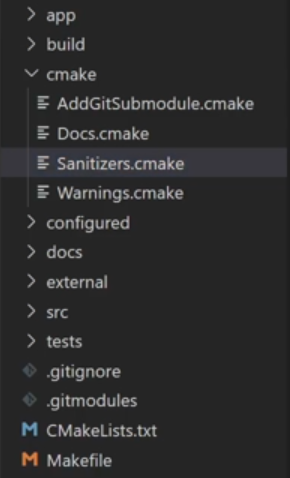
\includegraphics[width=2in]{san.png}
\end{center}


\subsection{Sanitizers.cmake}

In cmake directory, we have this file.


\begin{verbatim}
function(add_sanitizer_flags)
    if(NOT ${ENABLE_SANITIZE_UNDEF} AND NOT ${ENABLE_SANITIZE_ADDR})
        message(STATUS "Sanitizers deactivated") 
        return()
    endif()

    if(CMAKE_CXX_COMPILER_ID MATCHES "CLANG" OR CMAKE_CXX_COMPILER_ID MATCHES "GNU")
        add_compile_options("-fno-omit-frame-pointer")   
                                        # This functions adds compiler flags for every target
                                        # Sanitizers need to run on all of the application
        add_link_options("-fno-omit-frame-pointer")

        if (${ENABLE_SANITIZE_ADDR})
            add_compile_options("-fsanitize=address") 
            add_link_options("-fsanitize=address") 
        endif()

        if (${ENABLE_SANITIZE_UNDEF})
            add_compile_options("-fsanitize=undefined") 
            add_link_options("-fsanitize=undefined") 
        endif()

    elseif(CMAKE_CXX_COMPILER_ID MATCHES "MSVC")
        if (${ENABLE_SANITIZE_ADDR})
            add_compile_options("-fsanitize=address") 
            add_link_options("-fsanitize=address") 
        endif()

        if (${ENABLE_SANITIZE_UNDEF})
            message(STATUS "Undefined sanitizer is not implemented for MVSC")
        endif()

    else() 
        message(ERROR "Compiler not supported for Sanitizers")
    endif()
endfunction()
\end{verbatim}


\subsection{Activate Sanitizers in Root CMakeLists.txt}

Call the add\_sanitizer\_flags function from root.

\begin{verbatim}
if(ENABLE_SANITIZE_ADDR OR ENABLE_SANITIZE_UNDEF)
    include(Sanitizers)
    add_sanitizer_flags()
endif()
\end{verbatim}

\subsection{Sanitizer bug example}

Going out of bounds, like this, would be caught be clang-tidy, but not by compilers. Thus, Sanitizers help big time. See documentation at
gcc.gnu.org/onlinedocs/Instrumentation-Options.html.


\begin{center}
    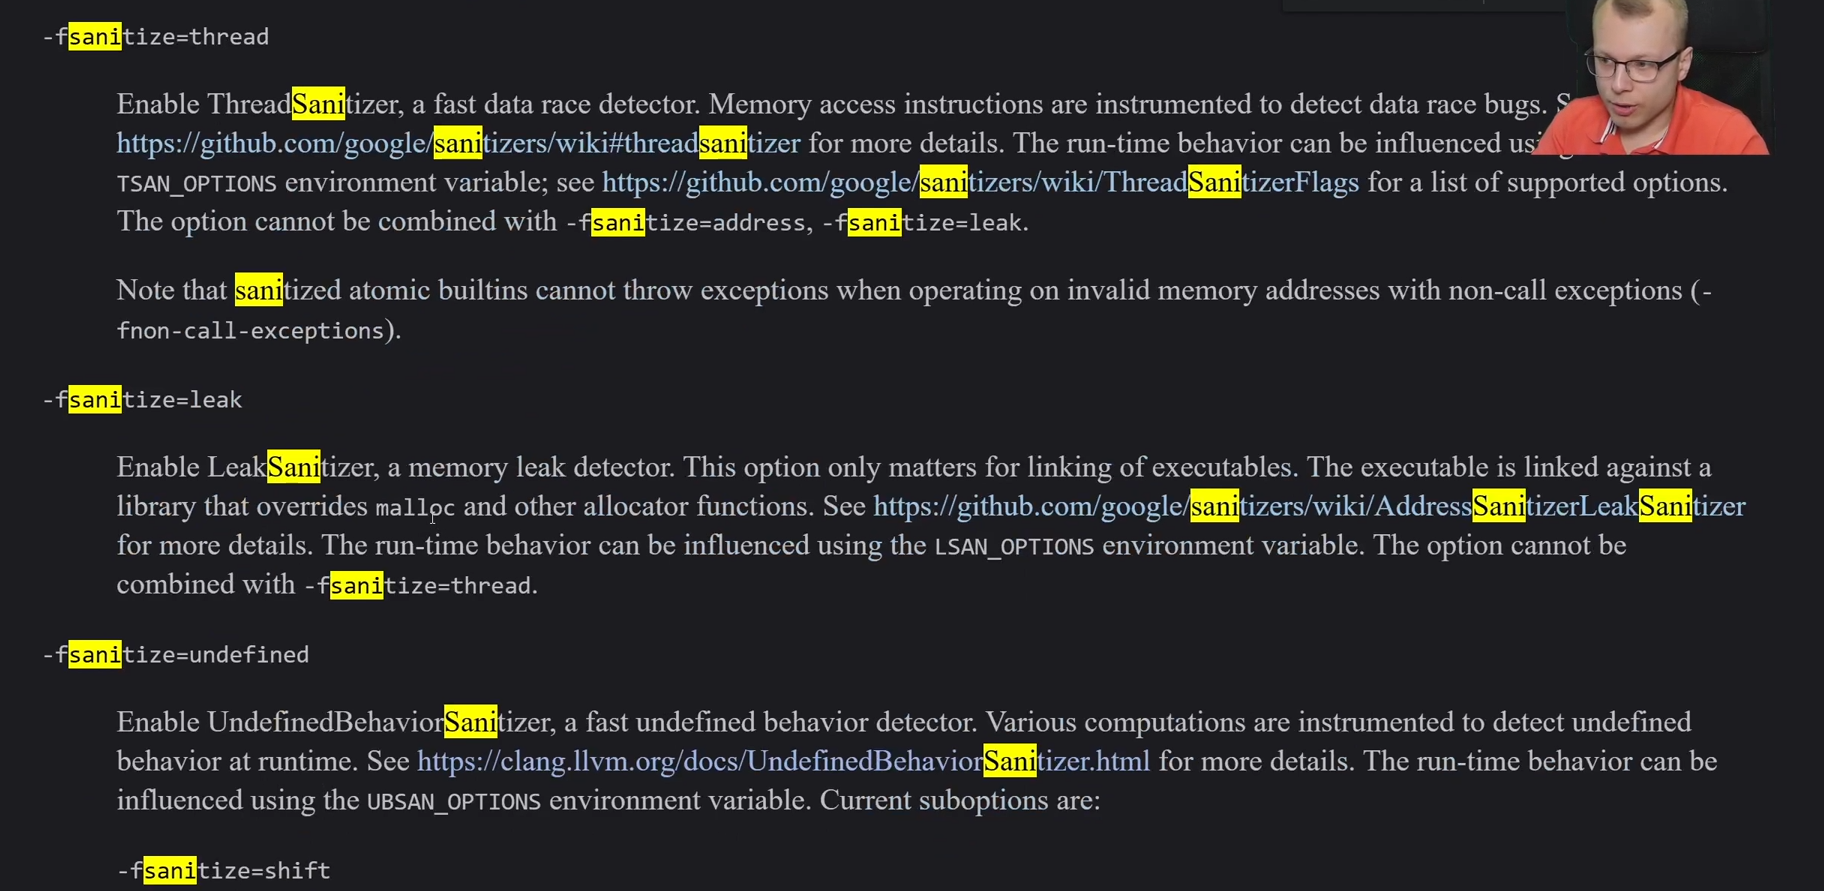
\includegraphics[width=5in]{fsan.png}
\end{center}


\begin{verbatim}
int main() {
    int x[2];
    x[2] = 1337;
}
\end{verbatim}

\section{IPO LTO}

In release mode, the release build, optimizations are activated to create the best product. C++ has many types of builds
for a project, debug modes, performance modes, etc. 

In this case, the release mode optimizations are related to the compiler for a better runtime. Yet, these optimizations
look at functions separately, not as a chain of functions so to speak (subsequent calls of different functions).

Link Time Optimization (LTO) or Interprocedural Optimization (IPO) [synonyms] is a response to these limits. Using functions from different translation units, the compiler with optimizations,
will be able to analyse them subsequently. In other words, the optimized compiler will be able to evaluate
if some operations can be cancelled in the function chain.

To use it, we will use a CMake function. All compilers (MSVC, CLANG and GCC) have LTO implemented.


\subsection{LTO Example - Clang}

\begin{verbatim}
--- a.h --- // .h for header file
            // this is genius note-taking!!!

extern int foo1(void);
extern void foo2(void);
extern void foo4(void);

--- a.c --- // .c for source file
            // this is genius note-taking!!!

#include "a.h"

static signed int i = 0;

void foo2(void {
    i = -1; 
}

static int foo3(void {
    i = -1; 
}

int foo1(void) {
    int data = 0;

    if (i < 0)
        data = foo3();

    data = data + 42;
    return data;
}

--- main.c ---
#include <stdio.h>
#include "a.h"

void foo4(void){
    printf("Hi\n");
}

int main() {
    return foo1()
}
\end{verbatim}

In this example, it is impossible for i to be reduced under zero. Since it is impossible, the foo3 function will never be
called. Thus, the compiler cancels an impossible chain and does not generate code for these logically uncallable functions.
This is the optimization.

\subsection{IPO LTO in CMake}

In your cmake directory, create a LTO.cmake file. Plus, create a new option in your root CMakelists.txt


\begin{verbatim}
option(ENABLE_LTO "Enable the link time optimization" ON)

...

if(ENABLE_LTO)
    include(LTO)
endif()
\end{verbatim}


\subsection{LTO.cmake}

Configuring link time optimization in the new lto.cmake file, in the cmake directory.

\begin{verbatim}
function(target_enable_lto TARGET ENABLE)
    if(NOT ${ENBALE})
    endif()

    include(CheckIPOSupported)
    check_ipo_supported(RESULT result OUTPUT output)

    if(result) 
        message(STATUS "IPO/LTO is supported!")
        set_property(TARGET ${TARGET} PROPERTY_INTERPROCEDURAL_OPTIMIZATION ${ENABLE})
    else()
        message("WARNING "IPO/LTO is not supported!")

                                     #PROPERTY... is a predefined variable in modern cmake
    endif()
endfunction(target_enable_lto)
\end{verbatim}


\subsection{In Our Target CMakeLists.txt}

Enabling LTO for our target library, means configuring it in its CMakeLists.txt file.

\begin{center}
    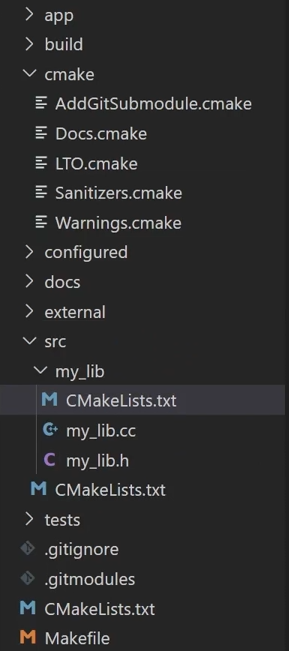
\includegraphics[width=2in]{lto_lib.png}
\end{center}


\begin{verbatim}
if(${ENABLE_LTO})
    target_enable_lto(${LIBRARY_NAME})
endif()

---- in app ----
---- CMakeLists.txt ----

if(${ENABLE_LTO})
    target_enable_lto(${EXECUTABLE_NAME} ${ENBALE_LTO})
endif()
\end{verbatim}


\section{Github Repositories}


\subsection{Cmake Scripts Update}


\subsection{Clang-Tidy}

 
\subsection{Clang-Format and CMake-Format}


\subsection{Github Pages}


\subsection{Code Coverage}


\subsection{Github Actions}


\subsection{Codecov}


\subsection{Pre-Commit}



\section{Starter Pack - Jason Turner's Template}

\begin{verbatim}
lefticus/cmake_template // Jason Turner 2023 cmake starter pack

rename "myproject" in the cmake files to use it.

\end{verbatim}

\subsection{Lefticus Defaults - ProjectOptions.cmake}

\begin{verbatim}
Address sanitizer
Undefined behavior sanitizer
Fuzzing example built
Procedural optimization IPO (link time optimization)
Warnings as errors
Clang-tidy enabled
CPPcheck enabled
Options for precompiled headers
\end{verbatim}

\subsection{Hardening - Hardening.cmake}

\begin{verbatim}
Hardened compilation // make code safer
More compilation options / securities.

-fstack-protector
-fcf-protection
-fsanitize=undefined // undefined behavior sanitizer
-fno-sanitize-recover=undefined
-fsanitizise-minimal-runtime

+ debug information 
\end{verbatim}

\section{Simple Cmake (Modern)}

\subsection{Context}

Cmake is "a generator of make files", it abstracts away makefile complexity.

\begin{verbatim}
First, cmake // generate make files
Second, make // run make files
Last, ./hello // run the created executable
\end{verbatim}

To create an executable of hello.cpp. We usually:
\begin{verbatim}
:wq // quit vim
g++ main.cpp -o hello // compile 
./hello // run the executable
\end{verbatim}

\subsection{CMakeLists.txt}

With Cmake, we can have:

\begin{verbatim}
// have cmake installed

cmake_minimum_required(VERSION 3.10)
set(CMAKE_CXX_STANDARD 17)
set(CMAKE_CXX_STANDARD_REQUIRED ON)

project(hello VERSION 1.0)
add_executable(hello main.cpp)
\end{verbatim}

Run CMake from the command line, specify a directory.
\begin{verbatim}
cmake . && make && ./hello
\end{verbatim}

\subsection{Cmake .  }

Generates all needed make files (Artifacts).

\begin{center}
    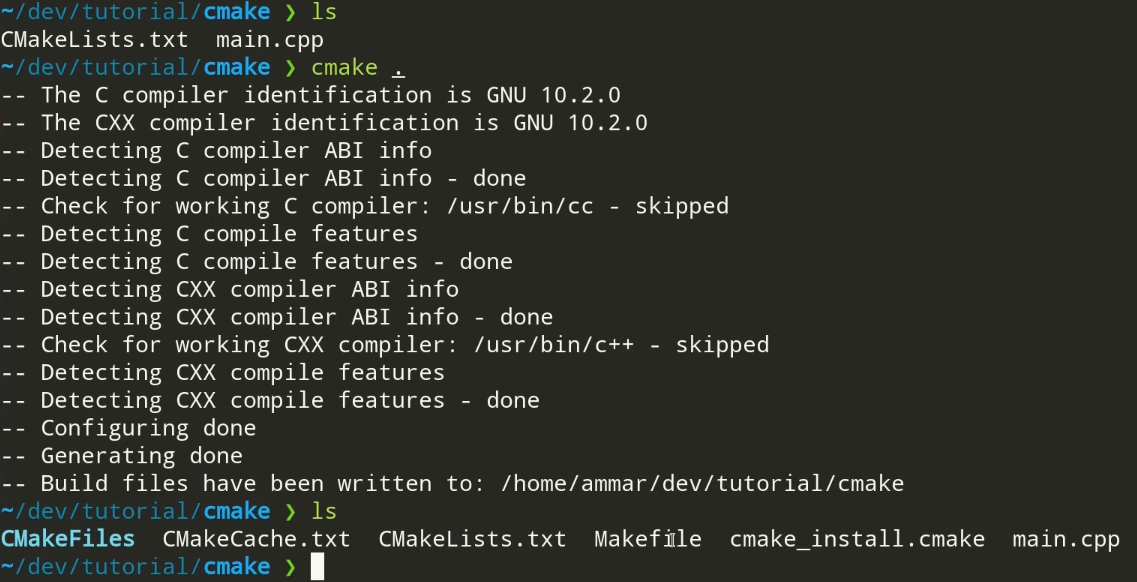
\includegraphics[width=4in]{cmake_dir.png}
\end{center}

\subsection{Make}

With the MakeFile generated by cmake. Build your binary (the executable) with:

\begin{center}
    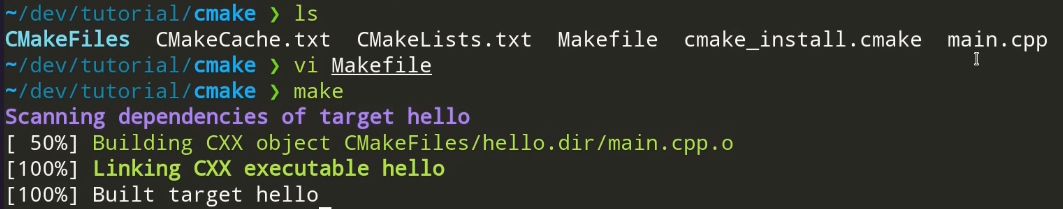
\includegraphics[width=4in]{make.png}
\end{center}

\subsection{Build folder}

\begin{center}
    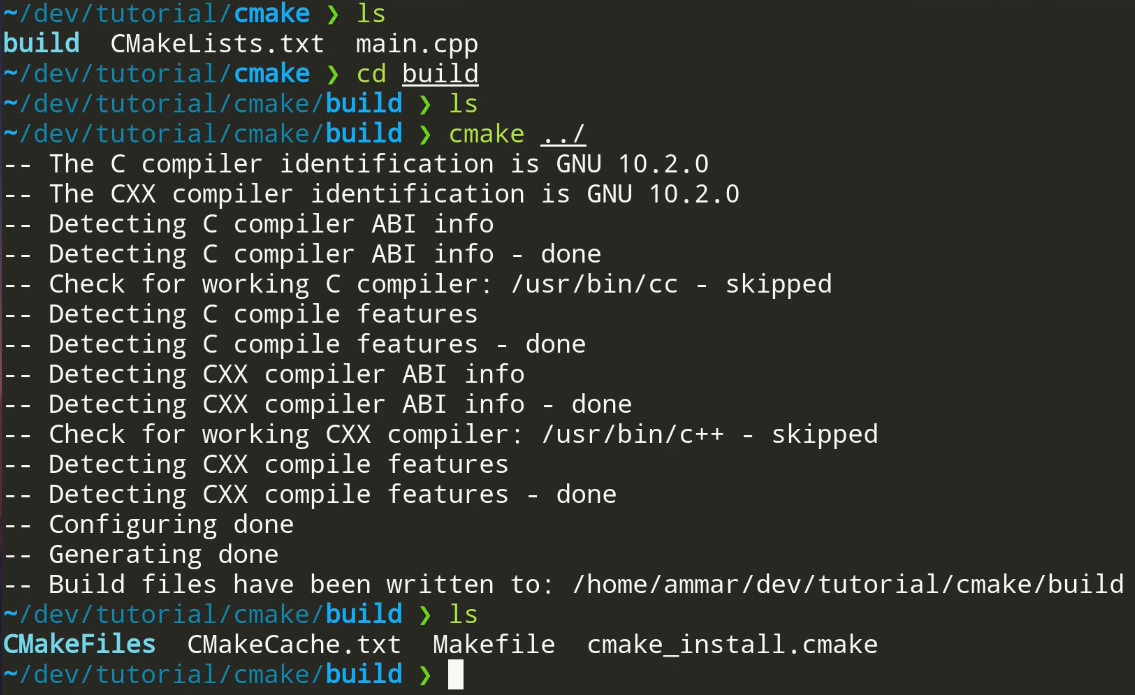
\includegraphics[width=4in]{build.png}
\end{center}

\subsection{Sick CMake Vim plugins combos}

\begin{verbatim}
See codevion/cpp2.md
\end{verbatim}

\subsection{COC - for code completion in nvim}
\begin{verbatim}
https://github.com/neoclide/coc.nvim
Jason Turner has this too
\end{verbatim}

\subsection{Include Header File - CMake Continued}

\begin{verbatim}
target_include_directories(hello PUBLIC ${CMAKE_CURRENT_SOURCE_DIR}/include)

    // Standard is having header files in /include directory!

hello // our target, where to add the stuff from headers
PUBLIC // gives the scope of added stuff from headers. 
       // Public, Private or Interface
       // Usage: when you have cmake library, make sure it is seen by #include in files

cmake_minimum_required(VERSION 3.10)
set(CMAKE_CXX_STANDARD 17)
set(CMAKE_CXX_STANDARD_REQUIRED ON)

project(hello VERSION 1.0)
add_executable(hello main.cpp)
target_include_directories(hello PUBLIC ${CMAKE_CURRENT_SOURCE_DIR}/include)
\end{verbatim}

\subsubsection{In header file}

\begin{verbatim}
#pragma once
#include <iostream>

class Blah {
    public:
        inline void boo() {
            std::cout << "Boo!\n";
        }
};
\end{verbatim}

\subsection{Pragma Once}

\begin{verbatim}
#pragma once is a non-standard directive that serves as an include guard. 
It ensures that a header file is included only once during the compilation process,
regardless of how many times it is referenced.

Placed at the beginning of a header file, it acts as a compiler directive to prevent multiple inclusions
Supported by most compilers, including GCC, Clang, and MSVC.
\end{verbatim}

\subsection{Glob - Include Many files with CMake}
 
You have at least two options. First, include every files one-by-one in the CMakeList.txt.
\begin{verbatim}
cmake_minimum_required(VERSION 3.10)
set(CMAKE_CXX_STANDARD 17)
set(CMAKE_CXX_STANDARD_REQUIRED ON)

project(hello VERSION 1.0) // traditional way to include files
add_executable(hello main.cpp Blah.cpp) // added here
target_include_directories(hello PUBLIC ${CMAKE_CURRENT_SOURCE_DIR}/include)
\end{verbatim}

Cmake discourages this glob method, but it is a more sane options for large projects.

\begin{verbatim}
file(GLOB_RECURSE SRC_FILES src/*.cpp) // glob everything in src/
add_executable(hello ${SRC_FILES})
\end{verbatim}

\subsection{src Directory - source files}

Declaration in the header file \textbf{blah.h}.
\begin{verbatim}
#pragma once

class Blah {
    public:
        void boo(); // declaring function boo in header
}
\end{verbatim}

Definition (implementation) of class Blah in the source files \textbf{blah.cpp}.
\begin{verbatim}
#include "blah.h"
#include <iostream>

void Blah::boo() {
    std::cout << "Boo!\n"; // defining function boo in src file
}
\end{verbatim}

\textbf{In CMake - Traditionally Added}
\begin{verbatim}
add_executable(hello main.cpp src/Blah.cpp) // added here
\end{verbatim}

\textbf{In CMake - Globing}
\begin{verbatim}
file(GLOB_RECURSE SRC_FILES src/*.cpp)
add_executable(hello main.cpp ${SRC_FILES})
\end{verbatim}

\subsection{CMake Custom Libraries}

Create a lib from some source files:

\begin{verbatim}
Replace add_executable with add_library

add_library(mylib STATIC lib/blah.cpp) // create a library
                                       // Staticly linked or dynamicly linked
\end{verbatim}

Then, include it in your main executable
\begin{verbatim}
target_link_libraries(hello Public mylib)
\end{verbatim}

\subsection{Custom Library Implementation - Blah example}

\begin{center}
    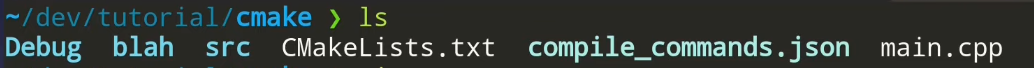
\includegraphics[width=2in]{blah_tree.png}
\end{center}

\begin{verbatim}
cmake_minimum_required(VERSION 3.10)
set(CMAKE_CXX_STANDARD 17)
set(CMAKE_CXX_STANDARD_REQUIRED ON)

project(hello VERSION 1.0)

add_library(blah STATIC blah/Blah.cpp)
target_include_directories(blah PUBLIC ${CMAKE_CURRENT_SOURCE_DIR}/blah/include)

// file(GLOB_RECURSE SRC_FILES src/*.cpp)
// now useless, since main.cpp has #include added library

// We are linking our library with our executable directly, with
// target_include_libraries

add_executable(hello main.cpp)
target_link_libraries(hello PUBLIC blah)
\end{verbatim}

The target link generates a libblah.a

\begin{center}
    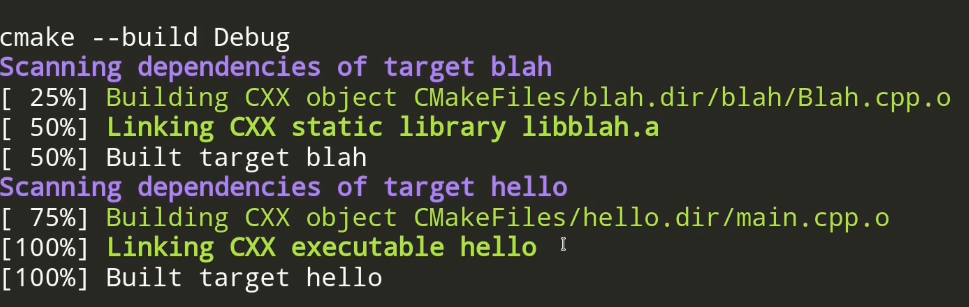
\includegraphics[width=2in]{target_link.png}
\end{center}

\section{Jason Turner's CMake Template - Options}

\begin{verbatim}
include(cmake/SystemLink.cmake)
include(cmake/LibFuzzer.cmake)
include(CMakeDependentOption)
include(CheckCXXCompilerFlag)

macro(myproject_supports_sanitizers)
  if((CMAKE_CXX_COMPILER_ID MATCHES ".*Clang.*" OR CMAKE_CXX_COMPILER_ID MATCHES ".*GNU.*") AND NOT WIN32)
    set(SUPPORTS_UBSAN ON)
  else()
    set(SUPPORTS_UBSAN OFF)
  endif()

  if((CMAKE_CXX_COMPILER_ID MATCHES ".*Clang.*" OR CMAKE_CXX_COMPILER_ID MATCHES ".*GNU.*") AND WIN32)
    set(SUPPORTS_ASAN OFF)
  else()
    set(SUPPORTS_ASAN ON)
  endif()
endmacro()

macro(myproject_setup_options)
  option(myproject_ENABLE_HARDENING "Enable hardening" ON)
  option(myproject_ENABLE_COVERAGE "Enable coverage reporting" OFF)
  cmake_dependent_option(
    myproject_ENABLE_GLOBAL_HARDENING
    "Attempt to push hardening options to built dependencies"
    ON
    myproject_ENABLE_HARDENING
    OFF)

  myproject_supports_sanitizers()

  if(NOT PROJECT_IS_TOP_LEVEL OR myproject_PACKAGING_MAINTAINER_MODE)
    option(myproject_ENABLE_IPO "Enable IPO/LTO" OFF)
    option(myproject_WARNINGS_AS_ERRORS "Treat Warnings As Errors" OFF)
    option(myproject_ENABLE_USER_LINKER "Enable user-selected linker" OFF)
    option(myproject_ENABLE_SANITIZER_ADDRESS "Enable address sanitizer" OFF)
    option(myproject_ENABLE_SANITIZER_LEAK "Enable leak sanitizer" OFF)
    option(myproject_ENABLE_SANITIZER_UNDEFINED "Enable undefined sanitizer" OFF)
    option(myproject_ENABLE_SANITIZER_THREAD "Enable thread sanitizer" OFF)
    option(myproject_ENABLE_SANITIZER_MEMORY "Enable memory sanitizer" OFF)
    option(myproject_ENABLE_UNITY_BUILD "Enable unity builds" OFF)
    option(myproject_ENABLE_CLANG_TIDY "Enable clang-tidy" OFF)
    option(myproject_ENABLE_CPPCHECK "Enable cpp-check analysis" OFF)
    option(myproject_ENABLE_PCH "Enable precompiled headers" OFF)
    option(myproject_ENABLE_CACHE "Enable ccache" OFF)
  else()
    option(myproject_ENABLE_IPO "Enable IPO/LTO" ON)
    option(myproject_WARNINGS_AS_ERRORS "Treat Warnings As Errors" ON)
    option(myproject_ENABLE_USER_LINKER "Enable user-selected linker" OFF)
    option(myproject_ENABLE_SANITIZER_ADDRESS "Enable address sanitizer" ${SUPPORTS_ASAN})
    option(myproject_ENABLE_SANITIZER_LEAK "Enable leak sanitizer" OFF)
    option(myproject_ENABLE_SANITIZER_UNDEFINED "Enable undefined sanitizer" ${SUPPORTS_UBSAN})
    option(myproject_ENABLE_SANITIZER_THREAD "Enable thread sanitizer" OFF)
    option(myproject_ENABLE_SANITIZER_MEMORY "Enable memory sanitizer" OFF)
    option(myproject_ENABLE_UNITY_BUILD "Enable unity builds" OFF)
    option(myproject_ENABLE_CLANG_TIDY "Enable clang-tidy" ON)
    option(myproject_ENABLE_CPPCHECK "Enable cpp-check analysis" ON)
    option(myproject_ENABLE_PCH "Enable precompiled headers" OFF)
    option(myproject_ENABLE_CACHE "Enable ccache" ON)
  endif()

  if(NOT PROJECT_IS_TOP_LEVEL)
    mark_as_advanced(
      myproject_ENABLE_IPO
      myproject_WARNINGS_AS_ERRORS
      myproject_ENABLE_USER_LINKER
      myproject_ENABLE_SANITIZER_ADDRESS
      myproject_ENABLE_SANITIZER_LEAK
      myproject_ENABLE_SANITIZER_UNDEFINED
      myproject_ENABLE_SANITIZER_THREAD
      myproject_ENABLE_SANITIZER_MEMORY
      myproject_ENABLE_UNITY_BUILD
      myproject_ENABLE_CLANG_TIDY
      myproject_ENABLE_CPPCHECK
      myproject_ENABLE_COVERAGE
      myproject_ENABLE_PCH
      myproject_ENABLE_CACHE)
  endif()

  myproject_check_libfuzzer_support(LIBFUZZER_SUPPORTED)
  if(LIBFUZZER_SUPPORTED AND (myproject_ENABLE_SANITIZER_ADDRESS OR myproject_ENABLE_SANITIZER_THREAD OR myproject_ENABLE_SANITIZER_UNDEFINED))
    set(DEFAULT_FUZZER ON)
  else()
    set(DEFAULT_FUZZER OFF)
  endif()

  option(myproject_BUILD_FUZZ_TESTS "Enable fuzz testing executable" ${DEFAULT_FUZZER})

endmacro()

macro(myproject_global_options)
  if(myproject_ENABLE_IPO)
    include(cmake/InterproceduralOptimization.cmake)
    myproject_enable_ipo()
  endif()

  myproject_supports_sanitizers()

  if(myproject_ENABLE_HARDENING AND myproject_ENABLE_GLOBAL_HARDENING)
    include(cmake/Hardening.cmake)
    if(NOT SUPPORTS_UBSAN 
       OR myproject_ENABLE_SANITIZER_UNDEFINED
       OR myproject_ENABLE_SANITIZER_ADDRESS
       OR myproject_ENABLE_SANITIZER_THREAD
       OR myproject_ENABLE_SANITIZER_LEAK)
      set(ENABLE_UBSAN_MINIMAL_RUNTIME FALSE)
    else()
      set(ENABLE_UBSAN_MINIMAL_RUNTIME TRUE)
    endif()
    message("${myproject_ENABLE_HARDENING} ${ENABLE_UBSAN_MINIMAL_RUNTIME} ${myproject_ENABLE_SANITIZER_UNDEFINED}")
    myproject_enable_hardening(myproject_options ON ${ENABLE_UBSAN_MINIMAL_RUNTIME})
  endif()
endmacro()

macro(myproject_local_options)
  if(PROJECT_IS_TOP_LEVEL)
    include(cmake/StandardProjectSettings.cmake)
  endif()

  add_library(myproject_warnings INTERFACE)
  add_library(myproject_options INTERFACE)

  include(cmake/CompilerWarnings.cmake)
  myproject_set_project_warnings(
    myproject_warnings
    ${myproject_WARNINGS_AS_ERRORS}
    ""
    ""
    ""
    "")

  if(myproject_ENABLE_USER_LINKER)
    include(cmake/Linker.cmake)
    configure_linker(myproject_options)
  endif()

  include(cmake/Sanitizers.cmake)
  myproject_enable_sanitizers(
    myproject_options
    ${myproject_ENABLE_SANITIZER_ADDRESS}
    ${myproject_ENABLE_SANITIZER_LEAK}
    ${myproject_ENABLE_SANITIZER_UNDEFINED}
    ${myproject_ENABLE_SANITIZER_THREAD}
    ${myproject_ENABLE_SANITIZER_MEMORY})

  set_target_properties(myproject_options PROPERTIES UNITY_BUILD ${myproject_ENABLE_UNITY_BUILD})

  if(myproject_ENABLE_PCH)
    target_precompile_headers(
      myproject_options
      INTERFACE
      <vector>
      <string>
      <utility>)
  endif()

  if(myproject_ENABLE_CACHE)
    include(cmake/Cache.cmake)
    myproject_enable_cache()
  endif()

  include(cmake/StaticAnalyzers.cmake)
  if(myproject_ENABLE_CLANG_TIDY)
    myproject_enable_clang_tidy(myproject_options ${myproject_WARNINGS_AS_ERRORS})
  endif()

  if(myproject_ENABLE_CPPCHECK)
    myproject_enable_cppcheck(${myproject_WARNINGS_AS_ERRORS} "" # override cppcheck options
    )
  endif()

  if(myproject_ENABLE_COVERAGE)
    include(cmake/Tests.cmake)
    myproject_enable_coverage(myproject_options)
  endif()

  if(myproject_WARNINGS_AS_ERRORS)
    check_cxx_compiler_flag("-Wl,--fatal-warnings" LINKER_FATAL_WARNINGS)
    if(LINKER_FATAL_WARNINGS)
      # This is not working consistently, so disabling for now
      # target_link_options(myproject_options INTERFACE -Wl,--fatal-warnings)
    endif()
  endif()

  if(myproject_ENABLE_HARDENING AND NOT myproject_ENABLE_GLOBAL_HARDENING)
    include(cmake/Hardening.cmake)
    if(NOT SUPPORTS_UBSAN 
       OR myproject_ENABLE_SANITIZER_UNDEFINED
       OR myproject_ENABLE_SANITIZER_ADDRESS
       OR myproject_ENABLE_SANITIZER_THREAD
       OR myproject_ENABLE_SANITIZER_LEAK)
      set(ENABLE_UBSAN_MINIMAL_RUNTIME FALSE)
    else()
      set(ENABLE_UBSAN_MINIMAL_RUNTIME TRUE)
    endif()
    myproject_enable_hardening(myproject_options OFF ${ENABLE_UBSAN_MINIMAL_RUNTIME})
  endif()

endmacro()
\end{verbatim}

\end{document}







